\section{Processi organizzativi}
    \subsection{Processi di coordinamento}
        \subsubsection{Comunicazione}
            In questa sezione vengono presentate le norme per la comunicazione tra le parti che aderiscono al progetto.
            \paragraph{Comunicazioni interne}
                Vengono di seguito esposte le metodologie di comunicazione all'interno del team Dream Corp.
                \newline
                Per le comunicazioni all'interno del gruppo viene utilizzato \textit{Slack}\pedice, un'applicazione di messaggistica multipiattaforma adatto per i gruppi di lavoro. Attraverso questo strumento è possibile suddividere lo spazio di comunicazione in canali tematici, ricercare messaggi, condividere file di grosse dimensioni e tracciare i messaggi.
                \newline
                All'interno di \textit{Slack} sono stati predisposti dei canali tematici al fine di rendere più efficiente lo scambio di messaggi:
                \begin{itemize}
                    \item \textbf{general}: Canale utilizzato per le comunicazioni e l'organizzazione di carattere generale;
                    \item \textbf{github-notificaton}: Canale a cui è stato aggiunto un bot di GitHub il quale permette di inviare un messaggio nel momento in cui un membro del team apre/chiude issues, effettua un merge o una \textit{push};
                    \item \textbf{automatismi}: Dove si discute dei software da utilizzare per creare automatismi;
                    \item \textbf{random}: Canale generico dove discutere di tutto ciò che non è inerente al progetto.    
                \end{itemize}
                
                ~\newline Inoltre sono stati predisposti dei canali per la redazione dei documenti, uno per ogni documento, in modo da facilitare la discussione degli stessi:
                \begin{itemize}
                    \item \textbf{norme\_di\_progetto}: Utilizzato per discutere delle norme di progetto da seguire durante lo sviluppo;
                    \item \textbf{piano\_progetto}: Canale riservato alla redazione del documento \textit{Piano di progetto};
                    \item \textbf{studio\_di\_fattibilita}: Canale per la raccolta delle considerazioni sui capitolati e per la scrittura del documento;
                    \item \textbf{piano\_di\_qualifica}: Utilizzato per discutere del raggiungimento della qualità e per l'organizzazione della redazione del documento;
                    \item \textbf{analisi\_requisiti}: Per discutere dei casi d'uso, requisiti e utilizzo del software per la redazione del documento \textit{Analisi dei requisiti}; 
                    \item \textbf{glossario}: Dove viene confrontato il contenuto dei glossari personali.
                \end{itemize}
                
                I membri del team sono tenuti a comunicare rispettando i topic, nel caso si volesse portare all'attenzione tutti i membri del gruppo sono presenti i comandi:
                \begin{itemize}
                    \item \textit{@everyone} per notificare tutti i membri del gruppo;
                    \item \textit{@channel} per notificare i membri di uno specifico canale.
                \end{itemize}
                
              
                Altre modalità di comunicazione previste sono:
                \begin{itemize}
                    \item Comunicazioni orali informali: per parlare di qualsiasi problematica, strategia, utilizzo di strumenti, consigli, dubbi;
                    \item Riunioni: Incontri di persona precedentemente organizzati.
                \end{itemize}        
            \paragraph{Comunicazioni esterne}
                Questa sezione è inerente alle modalità di comunicazione da seguire con i membri esterni al gruppo di lavoro.
                \newline
                Allo scopo di garantire un costante miglioramento della qualità di prodotto, sono stati individuati le seguenti entità esterne:
                \begin{itemize}
                    \item La proponente \textbf{Zucchetti S.p.a}, rappresentata da Gregorio Piccoli, board member e CTO dell'azienda, con il quale si vuole stabilire un rapporto di collaborazione per definire bisogni e requisiti per la realizzazione del prodotto;
                    \item I Committenti \textbf{Prof. Tullio Vardanega} e \textbf{Prof. Riccardo Cardin}, ai quali verrà consegnata tutta la documentazione in ciascuna fase di revisione, con i quali si vuole stabilire un rapporto utile al miglioramento dei processi e delle strategie.
                \end{itemize}
                \paragraph{Comunicazioni esterne scritte} Devono essere effettuate tassativamente attraverso l'uso dell'indirizzo mail del gruppo:
                \newline
                \begin{center}
                	\textit{dreamcorp.swe@gmail.com}
                \end{center}
                
    ~\newline Ogni email ricevuta a questo indirizzo verrà inoltrata automaticamente alla casella postale di ogni membro del gruppo attraverso l'utilizzo dei filtri di Gmail\pedice, inoltre il testo delle mail verrà riportato come messaggio su \textit{Slack} attraverso l'uso di un bot.
                \paragraph{Composizione email}
                Viene di seguito presentata la modalità di scrittura delle email rivolte a soggetti esterni.
                \begin{itemize}
    
                    \item \textbf{Email verso la Proponente Zucchetti S.p.a}: nel capitolato d'appalto viene fornita la mail del Dr. Gregorio Piccoli.
                    \begin{center}
                        \textit{gregorio.piccoli@zucchetti.it}
                    \end{center}
                         
                    Non sono state date direttive per la composizione dei messaggi, il gruppo si impegna a mantenere un formalismo nella comunicazione con l'azienda proponente.
                    \item \textbf{Email verso i Committenti}: ci si propone di utilizzare un oggetto che descriva in modo più accurato possibile il contenute del messaggio, ai committenti ci si rivolgerà con il Voi e con il Lei.
    
                \end{itemize}
                Nella possibilità in cui un messaggio debba essere mandato a più persone, nel campo "A:" va indicato il principale destinatario, mentre nel campo "Cc:" vanno indicati tutti gli altri.
                Viene posta particolare attenzione nella modalità di risposta e di inoltro delle email. In questi casi sono da utilizzare i tasti "Rispondi a tutti" e "Inoltra a" che formatteranno in automatico il corpo del messaggio includendo le clausole "Re:" e "I:".
                \subsubsection{Riunioni}
                    In questa sottosezione vengono presentate le modalità di riunione, sia interne che esterne.
                    Allo scopo di far rispettare l'ordine del giorno, redigere il \textit{Verbale di riunione} e prendere nota degli argomenti trattati e delle decisioni prese, all'interno di ogni riunione dovrà essere nominato a turno tra i membri del gruppo Dream Corp. un Segretario.
                    \paragraph{Verbali di riunione}
                       Nello svolgimento delle riunioni è compito del Segretario redigere il documento \textit{Verbale di riunione} secondo il seguente schema:
                        \begin{itemize}
                            \item \textbf{Verbale Esterno DATA}, incluso nel frontespizio. Per DATA si intende la data in cui è stata effettuata la riunione, scritta secondo le \textit{Norme Tipografiche};
                            \item \textbf{Informazioni sulla riunione}: sezione contenente:
                            \begin{itemize}
                                \item \textbf{Motivo}: Descrizione sintetica del motivo che ha portato ad indire una riunione;
                                \item \textbf{Luogo e Data}: ad esempio \textit{Padova, Giovedì 23 Febbraio 2019}; 
                                \item \textbf{Ora inizio}: nel formato ventiquattro ore;
                                \item \textbf{Ora fine}: nel formato ventiquattro ore;
                                \item \textbf{Partecipanti}: vengono elencati i partecipanti della riunione, iniziando dal Proponente/Committente nel caso la riunione sia esterna. Nel caso un membro sia costretto a lasciare la riunione prima del previsto, deve essere annotata l'ora di uscita e il motivo.
                            \end{itemize}
                            \item \textbf{Ordine del giorno}: Un elenco puntato degli argomenti discussi; 
                            \item \textbf{Resoconto}: sezione contente le annotazioni circa le decisioni prese con motivazioni e gli argomenti discussi e non.
                        \end{itemize}
                        \paragraph{Nomenclatura} 
                            I verbali esterni dovranno avere nome:
                            VER-DATA
                            \newline
                            I verbali interni saranno nominati:
                            VIR-DATA
                            \newline
                            Viene usata questa nomenclatura al fine di avere una facile consultazione.
                            \newline
                        \paragraph{Conservazione dei verbali}
                            I verbali interni ed esterni verranno redatti in \LaTeX e caricati nel repository del progetto.
                            Inoltre, in base alla natura del verbale, che può essere interna od esterna, il documento verrà posto nell'apposita cartella.
                    \paragraph{Riunioni interne}
                        La partecipazione delle riunioni interne è permessa ai soli membri del gruppo Dream Corp.
                        \newline
                        \paragraph{Compiti del Responsabile di Progetto}
                            Di seguito vengono elencati i compiti che deve eseguire il Responsabile di Progetto:
                            \begin{itemize}
                                \item Fissare la data delle riunioni interne, previa discussione con i membri all'interno del canale \textit{general} su \textit{Slack};
                                \item Stabilire l'ordine del giorno;
                                \item Valutare le richieste di riunione dei membri del gruppo e decidere se accettarle;
                                \item Comunicare data e ordine del giorno attraverso il comando \textbf{@everyone} all'interno di \textit{Slack} con almeno un giorno di anticipo;
                                \item Verificare ed approvare il verbale;
                                \item Confermare spostare od annullare le riunioni sempre con le modalità di notifica a tutti i membri del gruppo.
                             \end{itemize}
                         \paragraph{Compiti dei partecipanti}
                            \begin{itemize}
                                \item Comunicare tempestivamente assenze e/o ritardi; 
                                \item Presentarsi puntualmente alle riunioni;
                                \item Partecipare attivamente alle discussioni;
                                \item Mantenere un atteggiamento educato.
                            \end{itemize}
                        \paragraph{Approvazione delle decisioni}
                            Le decisioni vengono approvate con la regola della maggioranza dei partecipanti alla riunione.
                            Affinché una riunione sia valida devono essere presenti almeno cinque membri del gruppo.
                            
                      \paragraph{Riunioni esterne}
                      Fino al momento dell'approvazione di questo documento, non è stata effettuata nessuna riunione esterna e quindi questa sezione verrà specificata nelle future release di questo documento.
        \subsection{Processi di pianificazione}
            \subsubsection{Ruoli di progetto}
                Nonostante il progetto sia collaborativo, all'interno del gruppo sono stati assegnati dei ruoli corrispondenti alle figure aziendali, essi sono:
                \begin{itemize}
                    \item \textbf{Responsabile di progetto};
                    \item \textbf{Amministratore};
                    \item \textbf{Analista};
                    \item \textbf{Progettista};
                    \item \textbf{Programmatore};
                    \item \textbf{Verificatore}.
                \end{itemize}
                I ruoli verranno assegnati inizialmente verranno ruotati secondo un calendario prescritto nel documento \PdP.
                Si cercherà evitare situazioni di conflitto d'interesse, come per esempio attuare la verifica di un documento da parte del redattore dello stesso.
                \paragraph{Responsabile di Progetto}
                    La figura di "Project Manager", o Responsabile di progetto, è responsabile unico dell'avvio, pianificazione, esecuzione, controllo e chiusura di un progetto facendo ricorso a tecniche e metodi  di project management. Egli partecipa al progetto dall'inizio alla fine.
                    \newline
                    I compiti principali del Project Manager sono:
                    \begin{itemize}
                        \item Elaborare la pianificazione del lavoro;
                        \item Organizzare efficientemente ed efficacemente le risorse umane a sua disposizione;
                        \item Favorire la comunicazione e l'affiatamento del team di progetto;
                        \item Distribuire le risorse sulle attività e monitorarne lo svolgimento;
                        \item Prendere tutte le iniziative volte a prevenire i rischi;
                        \item Mantenere i contatti con gli utenti di riferimento e gli utenti finali pianificandone il coinvolgimento nelle varie attività del progetto;
                        \item Produrre la documentazione di sua competenza e supervisionare quella prodotta dal team di progetto;
                        \item Controllare la qualità dei prodotti parziali ed assicurarsi che gli standard di qualità adottati siano rispettati;
                        \item Avere sempre un'attenzione particolare al miglioramento dei processi produttivi del progetto.
                    \end{itemize}
                \paragraph{Amministratore}
                    L'Amministratore è colui che controlla l'ambiente di lavoro e che si preclude l'obiettivo di aumentare la qualità del lavoro dando strumenti al gruppo di lavoro.
                    I principali compiti dell'Amministratore sono:
                    \begin{itemize}
                        \item Amministrare le infrastrutture di supporto;
                        \item Risolvere i problemi riguardo la gestione dei processi;
                        \item Assicurare che la documentazione sia corretta, verificata, approvata, aggiornata e versionata;
                        \item Controllare le versioni e configurazioni dei prodotti;
                        \item Dare regole e procedure per lo svolgimento del lavoro.
                    \end{itemize}
                \paragraph{Analista}
                    L’attività dell'Analista è necessaria e fondamentale affinché il progetto possa essere realizzato. Il suo compito è quello di analizzare il dominio del problema per comprenderlo a pieno, abbassando le probabilità che vengano effettuati gravi problemi di progettazione. I suoi compiti comprendono:
                    \begin{itemize}
                        \item Lo studio e la definizione del problema da risolvere, per capire cosa deve essere realizzato e definire quindi gli accordi contrattuali in base ai requisiti richiesti;
                        \item La verifica delle implicazioni di costo e qualità;
                        \item La modellazione concettuale del sistema e la ripartizione dei requisiti;
                        \item La realizzazione dello Studio di fattibilità e dell’Analisi dei requisiti.
                    \end{itemize}
                \paragraph{Progettista}
                    Il Progettista è colui che redige il progetto, ha un proprio bagaglio culturale e una congrua esperienza. Egli:
                    \begin{itemize}
                        \item Concorre in prima persona allo sviluppo del progetto;
                        \item Supervisiona lo sviluppo software;
                        \item Controlla le attività svolte dal gruppo di lavoro;
                        \item Forma il personale e soggetti esterni.
                    \end{itemize}
                \paragraph{Programmatore}
                    Il Programmatore è una figura tecnica. Egli partecipa alla parte di codifica della realizzazione del prodotto. Egli:
                    \begin{itemize}
                        \item Scrive codice documentato e secondo le Norme di Progetto;
                        \item Predispone le componenti di supporto atte a verificare e validare il codice prodotto attraverso dei test;
                        \item Si occupa della stesura del \textit{Manuale Utente}.
                    \end{itemize}
                \paragraph{Verificatore}
                    I verificatori sono figure con competenze tecniche, esperienza professionale e conoscenza delle norme. Il Verificatore è presente per tutto lo svolgimento del progetto. I compiti sono:
                    \begin{itemize}
                        \item Assicurare che le \textit{Norme di Progetto} siano rispettate;
                        \item Controllare che ogni stadio di vita del prodotto sia conforme al \PdQ;
                        \item Segnala al Responsabile di Progetto eventuali situazioni di conflitto di interesse che violino la pianificazione stabilita nel \PdP.
                    \end{itemize}
                \subsubsection{Ticketing}
                    Attraverso l'Issue Tracking System di GitHub è possibile, in modo semplice e intuitivo, assegnare issues ai membri del gruppo.
                    I ticket rappresentano l’associazione di una issue ad un membro del gruppo. L’assegnazione dei ticket ad uno specifico componente del gruppo può avvenire secondo due modalità:
                    \begin{itemize}
                        \item \textbf{Pro-attivamente:} l’assegnatario dell' issue è già noto al momento della creazione dello stesso. In questo caso il ticket viene assegnato direttamente allo specifico componente del gruppo da parte del Responsabile di progetto;
                        \item \textbf{Retroattivamente:} nel caso di issue a bassa priorità oppure di grandi quantità di lavoro da parte di tutti i componenti del gruppo, può non essere possibile assegnare direttamente una issue ad un componente del gruppo. Queste issues possono essere assegnate autonomamente qualora il componente finisse in anticipo i ticket a lui già assegnati.\newline
                    \end{itemize}\clearpage
                    Il ciclo di vita di un ticket è illustrato nella seguente immagine:\newline
                    \begin{figure}[!htbp]
                    	    	\centering                 	    	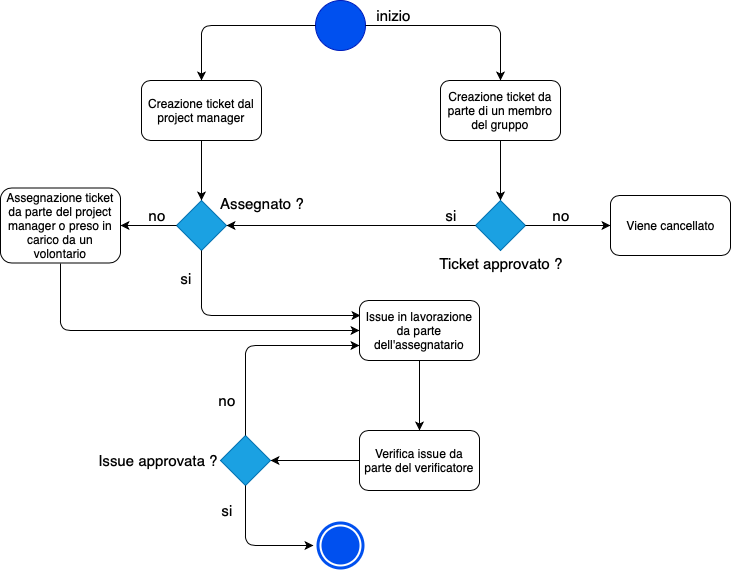
\includegraphics[scale=0.7]{lifeCycleTicket.png}
                    	    	\caption{Ciclo di vita del Ticket}
                    	    \end{figure}
                    
                    \clearpage
                    \paragraph{Struttura delle issues}
                        Le issues in GitHub hanno la seguente struttura:
                            \begin{itemize}
                                \item \textbf{Title}: Il titolo della issues che descrive il problema in generale;
                                \item \textbf{Write}: La descrizione dettagliata del problema;
                                \item \textbf{Assignes}: L'utente a cui è assegnato il compito di risolvere l'issue;
                                \item \textbf{Labels}: Etichetta con cui specificare la natura del problema;
                                \item \textbf{Projects}: Opzione che permette di assegnare una issue ad un progetto con relativa board;
                                \item \textbf{Milestone}: La milestone a cui assegnare l'issue. \newline
                            \end{itemize}
                            Inoltre una issue segue il seguente ciclo di vita:
                    	     \begin{figure}[!htbp]
                    	    	\centering
                    	    	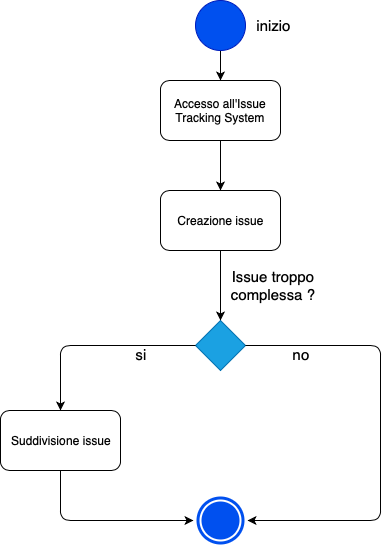
\includegraphics[scale=0.5]{task.png}
                    	    	\caption{Ciclo di vita della issue}
                    	    \end{figure}
                    	    \clearpage
                \subsubsection{Creazione dei diagrammi di Gantt}
                    Lo strumento scelto per la realizzazione dei diagrammi di Gantt\pedice è GanttProject,
                    in quanto è gratuito, open source, multipiattaforma ed è stato considerato adatto
                    ai nostri bisogni.
                \subsection{Formazione}            
                    \subsubsection{Formazione del personale}
                        I membri del gruppo Dream Corp. sono tenuti ad apprendere le tecnologie utilizzate per ogni ambito del progetto in modo autonomo usando le seguenti guide:
                    \begin{itemize}
                        \item \textbf{Grafana}: \url{http://docs.grafana.org/};
                        \item \textbf{JavaScript}: \url{https://www.w3schools.com/js/};
                        \item \textbf{JsBayes}: \url{https://github.com/vangj/jsbayes};
                        \item \textbf{Angular}: \url{https://angular.io/tutorial};
                        \item \textbf{InfluxDB}: \url{https://docs.influxdata.com/influxdb/v1.7/};
                        \item \textbf{Jest}: \url{https://jestjs.io/};
                        \item \textbf{WebPack}: \url{https://webpack.js.org/} .
                    \end{itemize}
                \subsection{Ambiente di lavoro}
                    \subsubsection{Coordinamento}
                        \paragraph{Versionamento} 
                            Per il versionamento si è scelto di utilizzare Git, soprattutto per il fatto che è stato utilizzato almeno una volta da tutti i componenti del gruppo. Ci si appoggia inoltre al sistema di hosting GitHub, che presenta un IssueTrackingSystem comodo ed efficace, oltre ad essere configurabile come bot di \textit{Slack}.
                        \paragraph{Pianificazione}
                            Per la pianificazione delle risorse è stato utilizzato GanttProject. I motivi che ci hanno portato a questa scelta sono:
                            \begin{itemize}
                                \item Creare tasks e milestones;
                                \item Creare baselines;
                                \item Organizzare i task con una struttura analitica.
                            \end{itemize}
                        \subsubsection{Documentazione}
                        \paragraph{\LaTeX} 
                            Per la scrittura di documenti si è scelto di utilizzare \LaTeX, un linguaggio di markup che permette di scrivere articoli ben formattati, oltre ad essere molto comodo per scrivere documenti in collaborazione con più persone, permettendo l'inclusione di più file all'interno come un vero e proprio linguaggio di programmazione.
                        \newline
                        \paragraph{Editor}
                            Come editor per la documentazione si è scelto di utilizzare OverLeaf, un servizio che permette l'editing dei testi online senza nessun tipo di installazione.
                        \subsubsection{Ambiente di sviluppo}
                            \paragraph{Sistemi operativi}
                                I membri del gruppo sono autorizzati ad utilizzare i più importanti sistemi operativi poiché supportano gli strumenti per la realizzazione del progetto.
                            \paragraph{IDE}
                                Poiché il linguaggio da utilizzare è JavaScript, si è scelto di utilizzare come IDE WebStorm essendo quello riconosciuto più adatto al linguaggio in questione.
                        \subsubsection{Ambiente di verifica}
                            \paragraph{Documenti} 
                                Per la verifica della correttezza della grammatica si è utilizzata la funzionalità di TexStudio che permette di effettuare il controllo ortografico del documento.
                           


                                 
                             
           
                         
                
                    
                     
                
            
    
     
            
            